\chapter{Security and Privacy}
\begin{figure}[htbp]
   \centering
   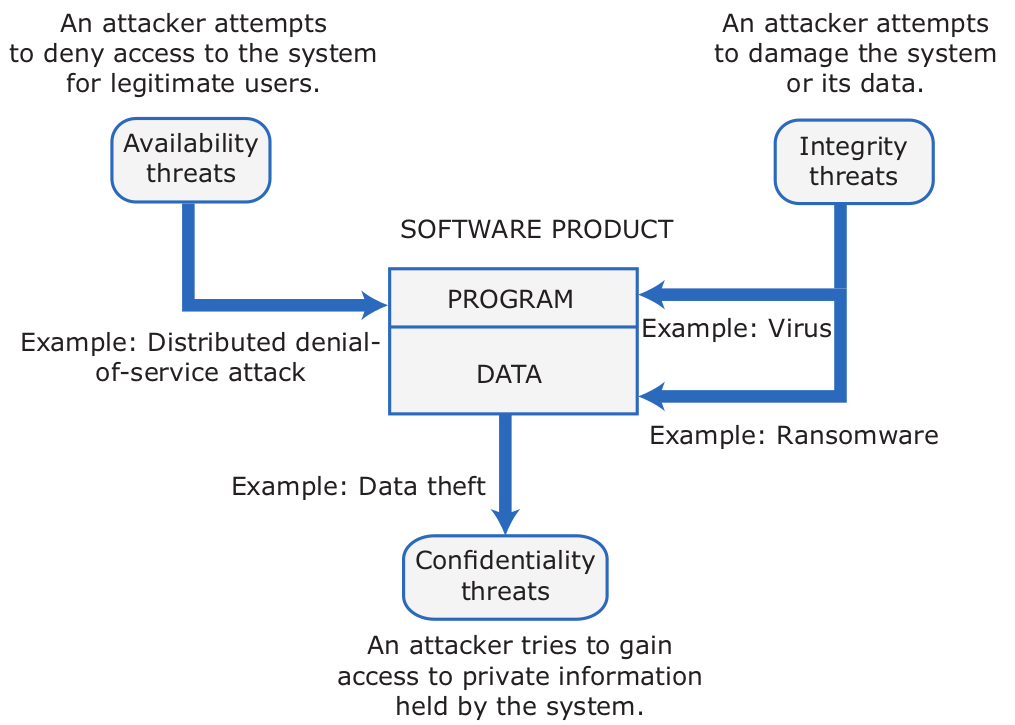
\includegraphics{images/security_threats.png}
   \caption{Security threats}
   \label{fig:security_threats}
\end{figure}

\section{Attacks types}

\subsection{Injection Attacks}
Malicious users try to crash the system by sending invalid input values.

\subsection{Session hijacking}
A \textit{Session} is a time period during which user's auth with a web app is valid;
it allows the user to not having to re-authenticate for subsequent system interactions.
A session is closed when the user logs out or due to a “times out” caused by
no user inputs for some time. 

\subsection{Cross-site Scripting}

\subsection{Denial-of-Service attacks}
\textbf{DoS} are intended to make system unavailable for normal use,
and were typically implemented by sending a high number of requests to overload servers,
resulting in the unavailability of services provided by such servers.

An historical \textbf{DoS} technique exploited the TCP 3-way handshake.
DoS developed in \textit{Distributed DoS} (\textbf{DDoS}),
i.e. sending requests from multiple IP addresses.

The most basic DoS techniques now have standard countermeasures to block them.
Widely used basic countermeasures include:
\begin{enumerate}
   \item IP tracking
   \item Temporary users lockout after failed authentication
\end{enumerate}

\subsection{Brute Force}
Attackers may try to guess missing authentication information by generating all possible combinations of characters,
possibly by knowing partial information on the string to be generated.


\section{Authentication}
\labelitemize{
   \textit{Approaches}
}{
   \begin{enumerate}
      \item \textbf{Knowledge}-based authentication\\
      Personal secret knwon by the user.\\
      Passwords are often insecure, forgotten, reused,
       and besides the user can be fooled into inserting it in fake websites (\textit{phishing}).
      \item \textbf{Possession}-based authentication\\
      Possessing a physical device which provides tokens.
      \item \textbf{Attribute}-based authentication\\
      Biometric information of the user.
      \item \textbf{Multi-factor}:\\
      Combining the above. 
      This is becoming way more common and standardized.
   \end{enumerate}
}

\section{Authorization}
\textbf{Authorization} involves checking that an authenticated user can \textit{access resources},
while \textbf{authentication} is only about ensuring that the user is who they claim to be.